\documentclass[11pt]{article}
\usepackage{amsmath, amssymb, amsfonts, amsthm}
\usepackage{geometry}
\geometry{letterpaper, margin=0.5in}
\usepackage{booktabs}
\usepackage{tikz}
\usepackage{hyperref}

\theoremstyle{definition} 
\newtheorem{definition}{Definition}[section]

\title{Pinned group summary: \texttt{SO(n=6, q=3)}}
\author{Pinning-Sympy automated output}
\date{\today}

\begin{document}

\maketitle
\tableofcontents

\newpage

\section{Basic group attributes}

\begin{tabular}{|l|l|}
	\hline
    Group & \texttt{SO(n=6, q=3)} \\
	\hline
    Matrix size & $6 \times 6$ \\
	\hline
    Rank & $3$ \\
	\hline
	Defining equations & $DefiningEquationPlaceholder$ \\
	\hline
\end{tabular}

\subsection{Symmetric bilinear form}
\begin{tabular}{|l|l|}
    \hline
    Dimension & 6 \\
    \hline
    Witt index & 3 \\
    \hline
    Primitive element & N/A \\
    \hline
    Epsilon & N/A \\
    \hline
\end{tabular}

\bigskip
\noindent Matrix: \(
\left[\begin{matrix}0 & 0 & 0 & 1 & 0 & 0\\0 & 0 & 0 & 0 & 1 & 0\\0 & 0 & 0 & 0 & 0 & 1\\1 & 0 & 0 & 0 & 0 & 0\\0 & 1 & 0 & 0 & 0 & 0\\0 & 0 & 1 & 0 & 0 & 0\end{matrix}\right]
\)



\subsection{Generic Lie algebra element}
\[
\left[\begin{matrix}x_{0 0} & x_{0 1} & x_{0 2} & 0 & - x_{1 3} & - x_{2 3}\\x_{1 0} & x_{1 1} & x_{1 2} & x_{1 3} & 0 & - x_{2 4}\\x_{2 0} & x_{2 1} & x_{2 2} & x_{2 3} & x_{2 4} & 0\\0 & - x_{4 0} & - x_{5 0} & - x_{0 0} & - x_{1 0} & - x_{2 0}\\x_{4 0} & 0 & - x_{5 1} & - x_{0 1} & - x_{1 1} & - x_{2 1}\\x_{5 0} & x_{5 1} & 0 & - x_{0 2} & - x_{1 2} & - x_{2 2}\end{matrix}\right]
\]

\subsection{Generic torus element}
\[
\left[\begin{matrix}t_{0} & 0 & 0 & 0 & 0 & 0\\0 & t_{1} & 0 & 0 & 0 & 0\\0 & 0 & t_{2} & 0 & 0 & 0\\0 & 0 & 0 & \frac{1}{t_{0}} & 0 & 0\\0 & 0 & 0 & 0 & \frac{1}{t_{1}} & 0\\0 & 0 & 0 & 0 & 0 & \frac{1}{t_{2}}\end{matrix}\right]
\]

\subsection{Trivial characters}
\[
\left[\begin{matrix}1 & 0 & 0 & 1 & 0 & 0\\0 & 1 & 0 & 0 & 1 & 0\\0 & 0 & 1 & 0 & 0 & 1\\1 & 1 & 1 & 1 & 1 & 1\end{matrix}\right]
\]

\newpage
\section{Root system}

\subsection*{Summary Properties}
\begin{tabular}{|l|l|}
    \hline
    Dynkin type & \texttt{A3} \\
    \hline
    Irreducible & True \\
    \hline
    Reduced & True \\
    \hline
    Simply laced & True \\
    \hline
    Number of roots & 12 \\
    \hline
\end{tabular}

\subsection{Dynkin diagram}
\begin{center}
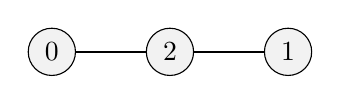
\begin{tikzpicture}[
    node/.style={circle, draw, fill=black!5, minimum size=6mm, inner sep=0pt},
    arrow/.style={-latex, thick},
    doublearrow/.style={double, double distance=2pt, -latex, thick},
    triplearrow/.style={double, double distance=4pt, -latex, thick},
    plain/.style={thick},
    baseline=(current bounding box.center)
]
    \node[node] (0) at (0.00, 0.00) {$0$};
    \node[node] (2) at (1.50, 0.00) {$2$};
    \node[node] (1) at (3.00, 0.00) {$1$};
    \draw[plain] (0) -- (2);
    \draw[plain] (1) -- (2);
\end{tikzpicture}
\end{center}

\subsection{Cartan matrix}
\[
\left[\begin{matrix}2 & 0 & -1\\0 & 2 & -1\\-1 & -1 & 2\end{matrix}\right]
\]

\subsection{Roots and coroots}
\begin{center}
\begin{tabular}{|l|l|c|c|c|}
    \hline
    \textbf{Root} & \textbf{Coroot} & \textbf{Simple} & \textbf{Sign} & \textbf{Multipliable} \\
    \hline
    $\left( -1, \  -1, \  0, \  0, \  0, \  0\right)$ & $\left( -1, \  -1, \  0, \  1, \  1, \  0\right)$ & No & $-$ & No \\
    \hline
    $\left( -1, \  0, \  -1, \  0, \  0, \  0\right)$ & $\left( -1, \  0, \  -1, \  1, \  0, \  1\right)$ & No & $-$ & No \\
    \hline
    $\left( -1, \  0, \  1, \  0, \  0, \  0\right)$ & $\left( -1, \  0, \  1, \  1, \  0, \  -1\right)$ & No & $-$ & No \\
    \hline
    $\left( -1, \  1, \  0, \  0, \  0, \  0\right)$ & $\left( -1, \  1, \  0, \  1, \  -1, \  0\right)$ & No & $-$ & No \\
    \hline
    $\left( 0, \  -1, \  -1, \  0, \  0, \  0\right)$ & $\left( 0, \  -1, \  -1, \  0, \  1, \  1\right)$ & No & $-$ & No \\
    \hline
    $\left( 0, \  -1, \  1, \  0, \  0, \  0\right)$ & $\left( 0, \  -1, \  1, \  0, \  1, \  -1\right)$ & No & $-$ & No \\
    \hline
    $\left( 0, \  1, \  -1, \  0, \  0, \  0\right)$ & $\left( 0, \  1, \  -1, \  0, \  -1, \  1\right)$ & Yes & $+$ & No \\
    \hline
    $\left( 0, \  1, \  1, \  0, \  0, \  0\right)$ & $\left( 0, \  1, \  1, \  0, \  -1, \  -1\right)$ & Yes & $+$ & No \\
    \hline
    $\left( 1, \  -1, \  0, \  0, \  0, \  0\right)$ & $\left( 1, \  -1, \  0, \  -1, \  1, \  0\right)$ & Yes & $+$ & No \\
    \hline
    $\left( 1, \  0, \  -1, \  0, \  0, \  0\right)$ & $\left( 1, \  0, \  -1, \  -1, \  0, \  1\right)$ & No & $+$ & No \\
    \hline
    $\left( 1, \  0, \  1, \  0, \  0, \  0\right)$ & $\left( 1, \  0, \  1, \  -1, \  0, \  -1\right)$ & No & $+$ & No \\
    \hline
    $\left( 1, \  1, \  0, \  0, \  0, \  0\right)$ & $\left( 1, \  1, \  0, \  -1, \  -1, \  0\right)$ & No & $+$ & No \\
    \hline
\end{tabular}
\end{center}


\subsection{Linear combinations of roots}

\begin{definition}
For two roots $\alpha, \beta$ in a root system $\Phi$, the set of positive integral linear combinations of $\alpha, \beta$ that are also roots is denoted
\(
	(\alpha, \beta) = \{ i \alpha + j \beta \in \Phi : i, j \in \mathbb{Z}_{\ge 1} \}
\)
\end{definition}

\begin{center}
\begin{tabular}{|l|l|c|}
    \hline
    $\alpha$ & $\beta$ & Pairs $(i,j)$ \\
    \hline
    $\left( -1, \  -1, \  0, \  0, \  0, \  0\right)$ & $\left( 0, \  1, \  -1, \  0, \  0, \  0\right)$ & $(1,1)$ \\
    \hline
    $\left( -1, \  -1, \  0, \  0, \  0, \  0\right)$ & $\left( 0, \  1, \  1, \  0, \  0, \  0\right)$ & $(1,1)$ \\
    \hline
    $\left( -1, \  -1, \  0, \  0, \  0, \  0\right)$ & $\left( 1, \  0, \  -1, \  0, \  0, \  0\right)$ & $(1,1)$ \\
    \hline
    $\left( -1, \  -1, \  0, \  0, \  0, \  0\right)$ & $\left( 1, \  0, \  1, \  0, \  0, \  0\right)$ & $(1,1)$ \\
    \hline
    $\left( -1, \  0, \  -1, \  0, \  0, \  0\right)$ & $\left( 0, \  -1, \  1, \  0, \  0, \  0\right)$ & $(1,1)$ \\
    \hline
    $\left( -1, \  0, \  -1, \  0, \  0, \  0\right)$ & $\left( 0, \  1, \  1, \  0, \  0, \  0\right)$ & $(1,1)$ \\
    \hline
    $\left( -1, \  0, \  -1, \  0, \  0, \  0\right)$ & $\left( 1, \  -1, \  0, \  0, \  0, \  0\right)$ & $(1,1)$ \\
    \hline
    $\left( -1, \  0, \  -1, \  0, \  0, \  0\right)$ & $\left( 1, \  1, \  0, \  0, \  0, \  0\right)$ & $(1,1)$ \\
    \hline
    $\left( -1, \  0, \  1, \  0, \  0, \  0\right)$ & $\left( 0, \  -1, \  -1, \  0, \  0, \  0\right)$ & $(1,1)$ \\
    \hline
    $\left( -1, \  0, \  1, \  0, \  0, \  0\right)$ & $\left( 0, \  1, \  -1, \  0, \  0, \  0\right)$ & $(1,1)$ \\
    \hline
    $\left( -1, \  0, \  1, \  0, \  0, \  0\right)$ & $\left( 1, \  -1, \  0, \  0, \  0, \  0\right)$ & $(1,1)$ \\
    \hline
    $\left( -1, \  0, \  1, \  0, \  0, \  0\right)$ & $\left( 1, \  1, \  0, \  0, \  0, \  0\right)$ & $(1,1)$ \\
    \hline
    $\left( -1, \  1, \  0, \  0, \  0, \  0\right)$ & $\left( 0, \  -1, \  -1, \  0, \  0, \  0\right)$ & $(1,1)$ \\
    \hline
    $\left( -1, \  1, \  0, \  0, \  0, \  0\right)$ & $\left( 0, \  -1, \  1, \  0, \  0, \  0\right)$ & $(1,1)$ \\
    \hline
    $\left( -1, \  1, \  0, \  0, \  0, \  0\right)$ & $\left( 1, \  0, \  -1, \  0, \  0, \  0\right)$ & $(1,1)$ \\
    \hline
    $\left( -1, \  1, \  0, \  0, \  0, \  0\right)$ & $\left( 1, \  0, \  1, \  0, \  0, \  0\right)$ & $(1,1)$ \\
    \hline
    $\left( 0, \  -1, \  -1, \  0, \  0, \  0\right)$ & $\left( 1, \  0, \  1, \  0, \  0, \  0\right)$ & $(1,1)$ \\
    \hline
    $\left( 0, \  -1, \  -1, \  0, \  0, \  0\right)$ & $\left( 1, \  1, \  0, \  0, \  0, \  0\right)$ & $(1,1)$ \\
    \hline
    $\left( 0, \  -1, \  1, \  0, \  0, \  0\right)$ & $\left( 1, \  0, \  -1, \  0, \  0, \  0\right)$ & $(1,1)$ \\
    \hline
    $\left( 0, \  -1, \  1, \  0, \  0, \  0\right)$ & $\left( 1, \  1, \  0, \  0, \  0, \  0\right)$ & $(1,1)$ \\
    \hline
    $\left( 0, \  1, \  -1, \  0, \  0, \  0\right)$ & $\left( 1, \  -1, \  0, \  0, \  0, \  0\right)$ & $(1,1)$ \\
    \hline
    $\left( 0, \  1, \  -1, \  0, \  0, \  0\right)$ & $\left( 1, \  0, \  1, \  0, \  0, \  0\right)$ & $(1,1)$ \\
    \hline
    $\left( 0, \  1, \  1, \  0, \  0, \  0\right)$ & $\left( 1, \  -1, \  0, \  0, \  0, \  0\right)$ & $(1,1)$ \\
    \hline
    $\left( 0, \  1, \  1, \  0, \  0, \  0\right)$ & $\left( 1, \  0, \  -1, \  0, \  0, \  0\right)$ & $(1,1)$ \\
    \hline
\end{tabular}
\end{center}


\section{Root spaces}

\begin{center}
\begin{tabular}{|l|c|}
\hline
Root & Dimension \\
\hline
$\left( -1, \  -1, \  0, \  0, \  0, \  0\right)$ & $1$ \\
\hline
$\left( -1, \  0, \  -1, \  0, \  0, \  0\right)$ & $1$ \\
\hline
$\left( -1, \  0, \  1, \  0, \  0, \  0\right)$ & $1$ \\
\hline
$\left( -1, \  1, \  0, \  0, \  0, \  0\right)$ & $1$ \\
\hline
$\left( 0, \  -1, \  -1, \  0, \  0, \  0\right)$ & $1$ \\
\hline
$\left( 0, \  -1, \  1, \  0, \  0, \  0\right)$ & $1$ \\
\hline
$\left( 0, \  1, \  -1, \  0, \  0, \  0\right)$ & $1$ \\
\hline
$\left( 0, \  1, \  1, \  0, \  0, \  0\right)$ & $1$ \\
\hline
$\left( 1, \  -1, \  0, \  0, \  0, \  0\right)$ & $1$ \\
\hline
$\left( 1, \  0, \  -1, \  0, \  0, \  0\right)$ & $1$ \\
\hline
$\left( 1, \  0, \  1, \  0, \  0, \  0\right)$ & $1$ \\
\hline
$\left( 1, \  1, \  0, \  0, \  0, \  0\right)$ & $1$ \\
\hline
\end{tabular}\end{center}

RootSpaceTablePlaceholder

\section{Root subgroups}

RootSubgroupTablePlaceholder

HomomorphismDefectTablePlaceholder

HomomorphismDefectIdentitiesPlaceholder

\section{Commutators}

CommutatorCoefficientTablePlaceholder

CommutatorIdentitiesPlaceholder

\section{Weyl group}

WeylGroupPlaceholder

WeylConjugationCoefficientPlaceholder

WeylConjugationIdentitiesPlaceholder

\section{Coroot torus elements ($h_\alpha$)}

CorootTorusElementPlaceholder

\end{document}